%Put this in order they appear in beamline?
\section{Beamline Components}

When the electrons from the CEBAF Accelerator have circulated the desired number of passes, they then enter the Hall A beamline. The Hall A Beamline has several measurement devices that allow the experimenter to fully understand the beam that is being delivered to the hall. A schematic of Hall A with the beamline components that are present in the hall can be seen in Figure \ref{fig:ha_overhead}. High beam quality and understanding the beams characteristics are critical for accurate analysis of an experiment. In the MARATHON experiment, the critical beamline components (which will be described in this section) are:

\begin{itemize}
	\item Beam Arc Energy Measurement
	\item Beam Current Monitor
	\item Raster
	\item Beam Position Monitor
\end{itemize}

\begin{figure}[h]
\begin{center}
	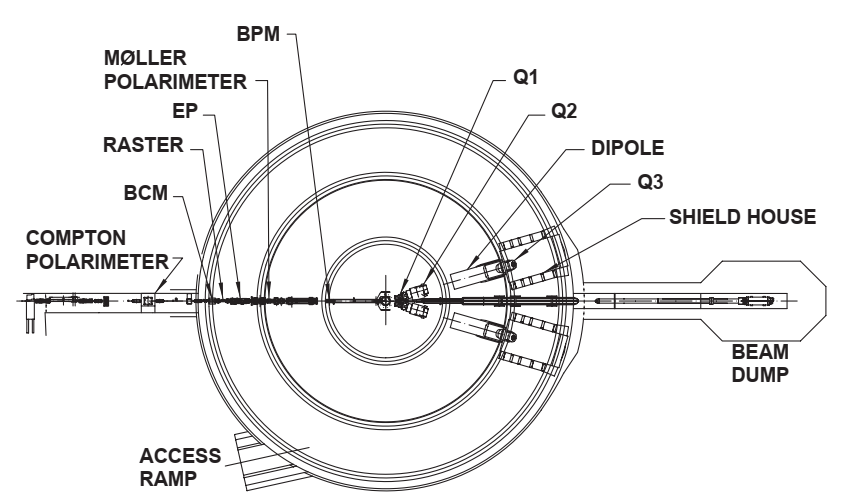
\includegraphics[width=0.7\textwidth]{./setup/fig/HallA_overhead.png}
	\caption{An overhead schematic of Hall A \cite{HANIM}.}
	\label{fig:ha_overhead}
\end{center}
\end{figure}

\subsection{Arc Energy Measurement}

Knowing the energy of the beam into the hall is critical for understanding the kinematics of the scattered electrons. This is done by measuring the deflection of the beam when passing through a series of eight dipoles in the beam arc leading to the hall. This measurement requires wire scanners to measure the bend angle of the beam through the arc and a probe to measure the magnetic field integral of the dipole magnets. 

The wire scanners are ``harps'' in the beamline, two before and two after the arc. A harp consists of three tungsten wires that are introduced sequentially into the path of the beam using a stepper motor. When the beam is incident on a wire, an electromagnetic shower is induced on the wire which is read by a PMT. By determining when each wire is struck by the beam, the position of the beam can be determined very accurately. Using two harps in each position also allows for beam direction measurement. Using a harp is a destructive measurement. 

\begin{figure}[h]
\begin{center}
	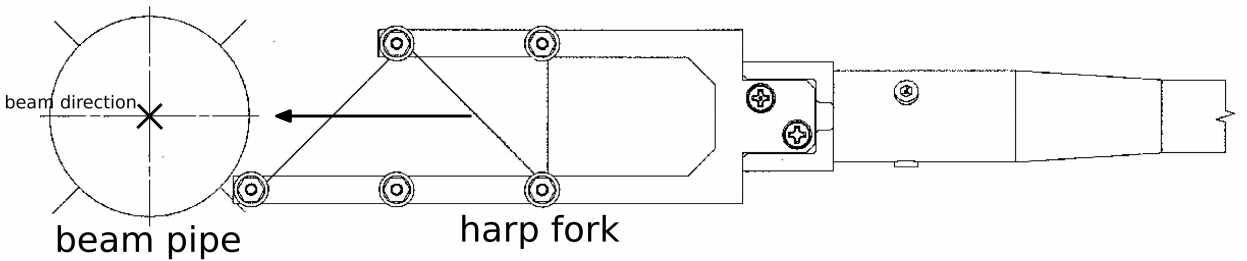
\includegraphics[width=\textwidth]{./setup/fig/harp.png}
	\caption{A schematic drawing of a harp scanner. The harp is introduced into the beamline with a stepper motor. The three wires create a signal when they interact with the beam, allowing for highly accurate beam position determination. The wires touching the beam is a destructive measurement \cite{harp_schem}.}
\end{center}
\end{figure}

The field integral is measured on a ninth reference dipole that is not in the beamline. This ninth dipole is identical to the eight dipoles in the arc and is powered in series with the other dipoles. Measuring the field integral of the dipole requires a probe to be within the magnet, necessitating the use of this reference magnet \cite{HASEM}.

After measuring the field integral $\int\vec{B}\cdot\vec{d}l$ (in Tm) and angle $\theta$ (in radians), the momentum (in GeV/$c$) can be calculated with
\begin{equation}
	p = k\frac{\int\vec{B}\cdot\vec{d}l}{\theta}
\end{equation}
where $k=0.299792$ GeV$\cdot$rad/$\left(\text{Tm}c\right)$.

\subsection{Beam Current Monitor}

The Hall A Beam Current Monitor (BCM) is comprised of an Unser monitor and two RF cavities. The Unser, a Parametric Current Transformer, provides an absolute reference for the RF cavities. Each RF cavity is tuned to the frequency of the beam (1.497 GHz). The resonance then produces a voltage proportional to the beam current. The signals are then split to be either sampled or integrated. The sampled signal outputs the RMS of the voltage over a 1 second period. This is equivalent to the average beam current for that second. The signal that is integrated is first sent to an RMS-to-DC converter which is then fed to a Voltage-to-Frequency converter. This signal is then sent to a scalar that accumulates over a run. The final scalar value is proportional to the total accumulated charge in the run.

\subsubsection{Beam Current Monitor Calibration}

The Unser is calibrated by putting a current on a wire that is inside of the Unser cavity and measuring the signal that is output. The calibration of the Unser drifts quite quickly, so it is used to calibrate the RF cavities but cannot be used for long-term monitoring. Once the Unser is properly calibrated, the reading can be used to determine the calibration for the RF cavities. The RF cavity calibration is a linear relationship between the RF cavity reading and the beam current.

\subsection{Raster}

\begin{figure}[h]
\begin{center}
	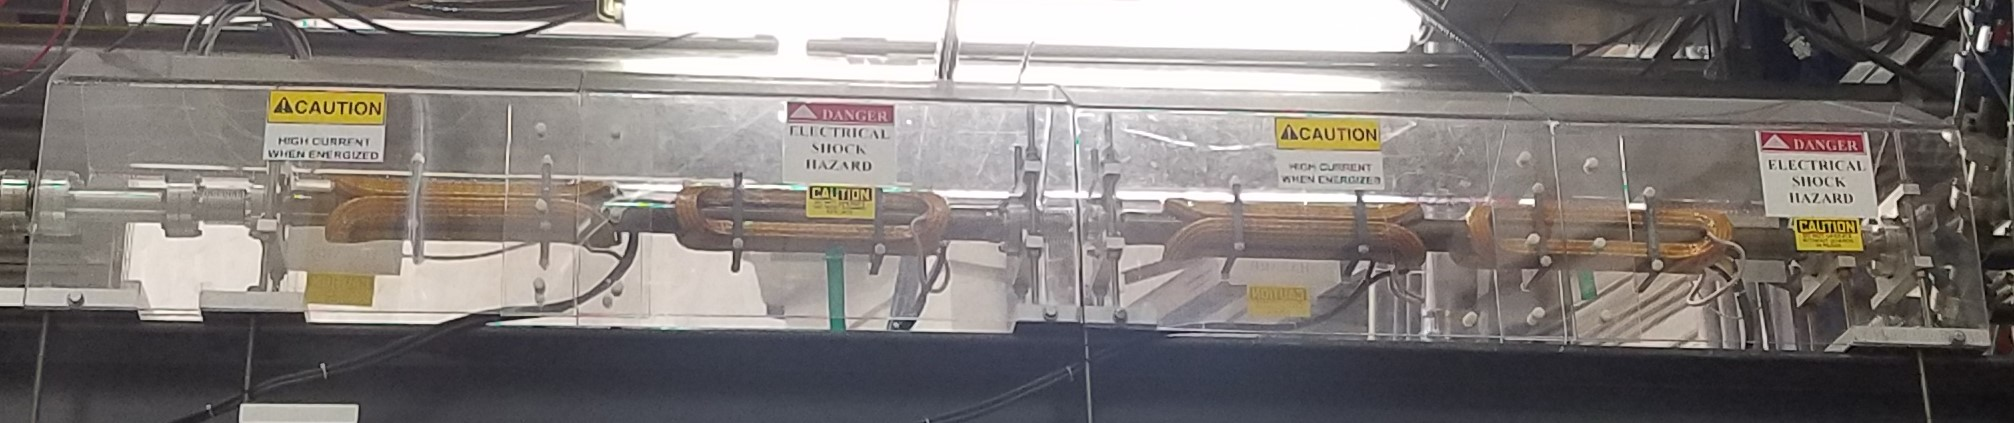
\includegraphics[width=\textwidth]{./setup/fig/raster_pic.jpg}
	\caption{The Hall A raster consists of four dipole magnets on the beamline}
	\label{fig:rasterpic}
\end{center}
\end{figure}

When the beam enters Hall A, it has very little spread, meaning that all of the electrons will strike the target in one small location (typically 80-200 $\mu$m). This poses an issue for the targets in use. Depending on the beam current in use, a localized beam spot can significantly heat up the target. In the case of solid targets, this risks melting the target. For gas targets, there is a potential for cell rupture. The raster, shown in Figure \ref{fig:rasterpic}, exists in the beamline to mitigate this risk by spreading the beam over a larger area on the target. The larger beam spread helps to reduce localized heating of the target due to the incident beam. The raster is a set of four dipole magnets: two for steering horizontally (x) and two for steering vertically (y) \cite{Bob}.

\begin{figure}[h]
\begin{center}
	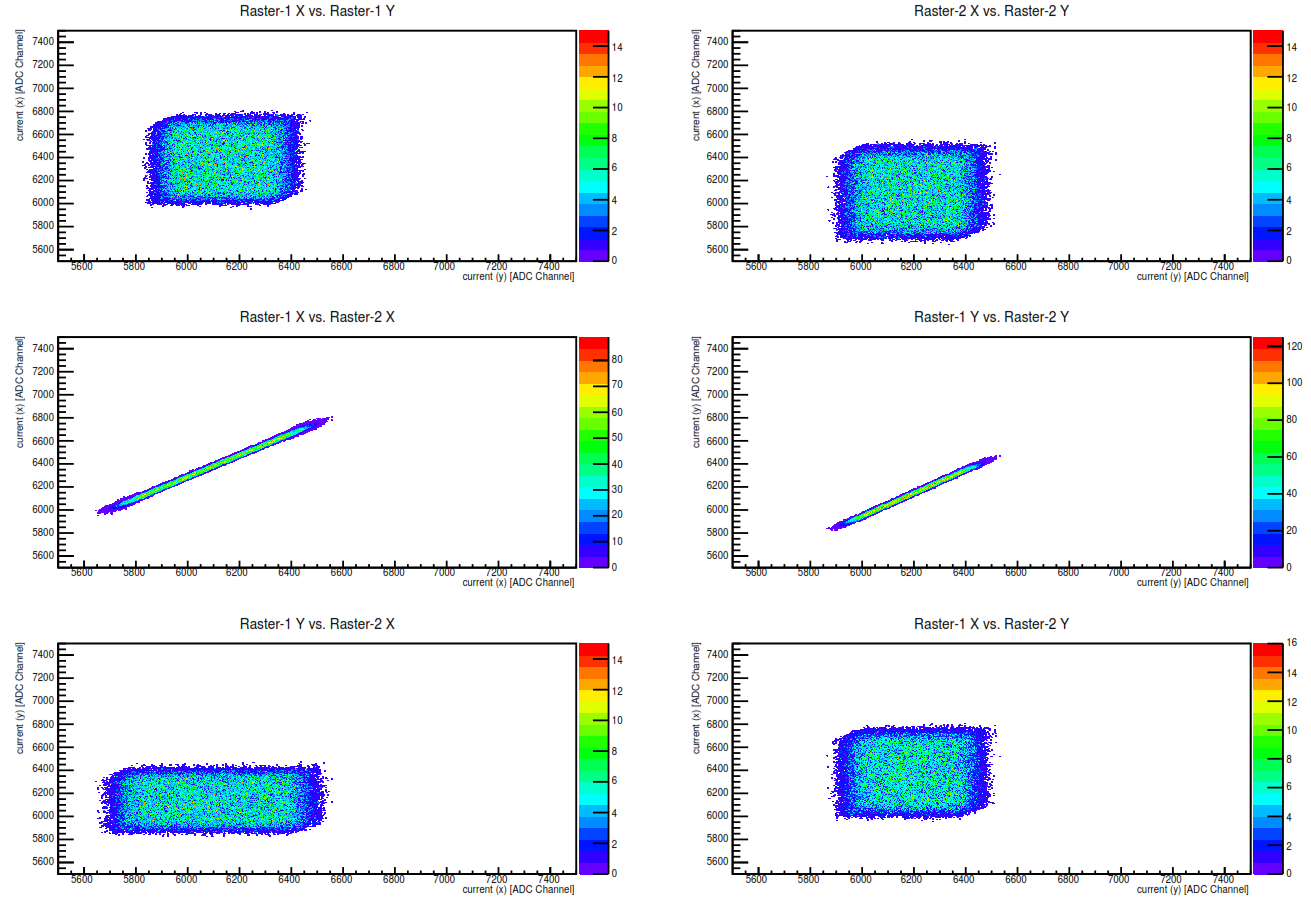
\includegraphics[width=0.7\textwidth]{./setup/fig/raster_sync.png}
	\caption{The X and Y raster pairs are each synced to produce the maximum kick. The X and Y directions are uncorrelated so that the beam travels uniformly over the target.}
	\label{fig:raster}
\end{center}
\end{figure}

\begin{figure}[h!]
\begin{center}
	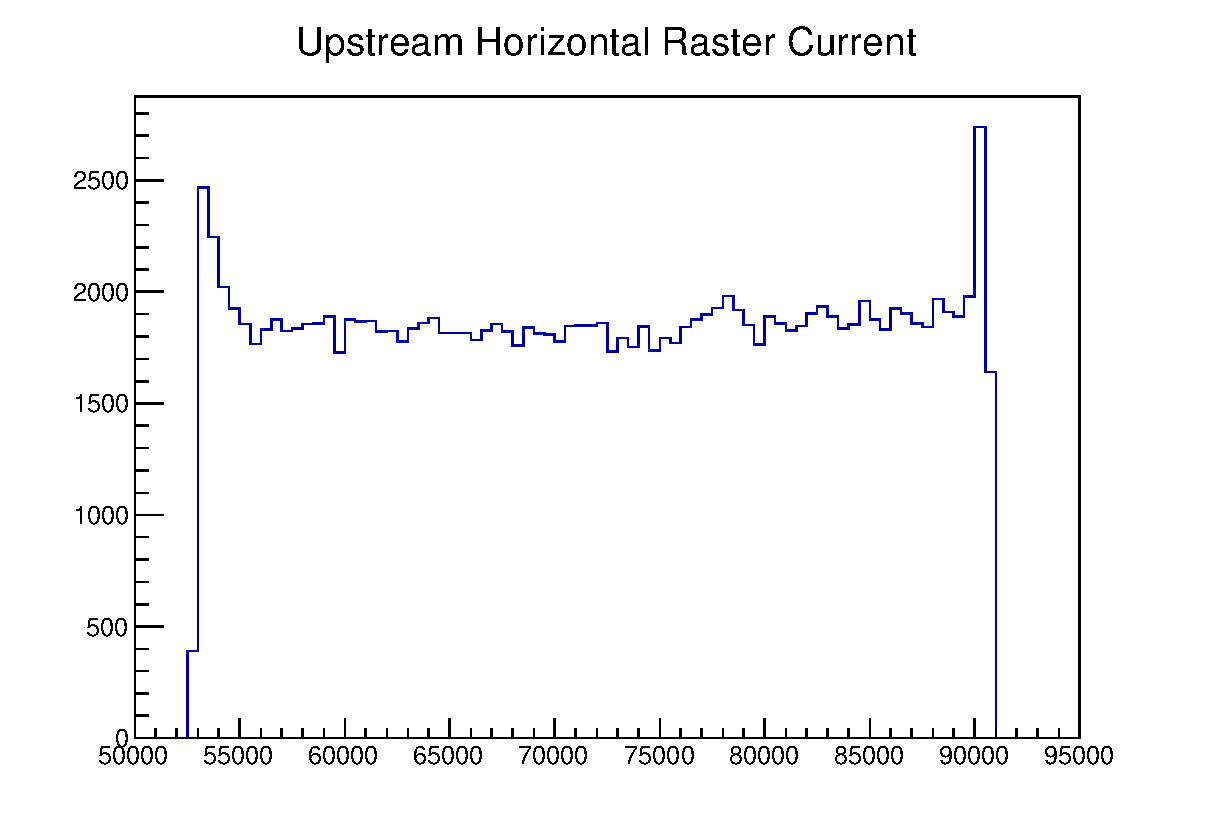
\includegraphics[width=0.7\textwidth]{./setup/fig/ex_rast.eps}
	\caption{An example of a raster current spectrum. The range and size will change with ADCs used, beam energy, and raster size. The shape should always stay the same. The ``bedposts'' on the edges are due to rounding of the triangular waveform by a low-pass filter.}
	\label{fig:exrast}
\end{center}
\end{figure}

The magnet pairs that work in the same direction are synced, which ensures that they maximize the beam spread and do not work against each other. This characteristic can be seen in Figure \ref{fig:raster}. Each raster magnet is powered by a triangle wave of different frequencies to minimize harmonics. The horizontal rasters are set to 24.5 kHz and the vertical rasters are set to 25 kHz \cite{rast_current}. The triangle wave ensures that equal time is spent at all points in the rastered area. Figure \ref{fig:exrast} shows a typical raster spectrum as recorded by the High Resolution Spectrometer (HRS).

\subsubsection{Raster Calibration}

The raster is calibrated by defining a line that maps the raster current to positions at each BPM and the target. To do this, the slope and intercept of this line had to be determined. The slope corresponds to the conversion of raster current to position displacement. The intercept is then determined from the central position that the beam is displaced from. This section will be a general presentation of the techniques used to calibrate the raster. For a more in-depth discussion of how the raster was calibrated, see Appendix \ref{raster_appendix}.

For the horizontal raster, this was done by optimizing the reconstructed z-vertex on the target. When properly calibrated, there should be no correlation between the horizontal raster and the z-vertex. Linear interpolation between two ``bad'' calibrations is a simple way to determine the correct calibration slope.

The veritcal raster could be calibrated in a similar way by minimizing the correlation between the vertical raster and a known momentum phenomena (i.e. a $W^2$ peak). Unfortunately, such a feature does not exist within the kinematics of MARATHON data. The vertical calibration was determined using the carbon hole target. The hole is known to be $2$mm diameter. By using the raster data, the hole can be fit in order to determine the vertical calibration slope.

The intercepts are determined by looking at the mean BPM position readings and projecting these to the target. This position will correspond to the mean value of the rasters as well. Using the beam position, raster current, and calibration slope the calibration intercept can easily be determined.

\subsection{Beam Position Monitors}

The Beam Position Monitors (BPMs) are a pair of measurement devices that consist of four sensing wires, as diagrammed in Figure \ref{fig:bpm}. These four sensing wires are tuned to the fundamental frequency of the beam. Using the signal received from each wire, the experimenter can reconstruct the position of the beam as it passed the BPM. Using both BPMs in conjunction allows the experimenter to determine the beam trajectory and where the electrons are incident on the target.

\begin{figure}[h]
\begin{center}
	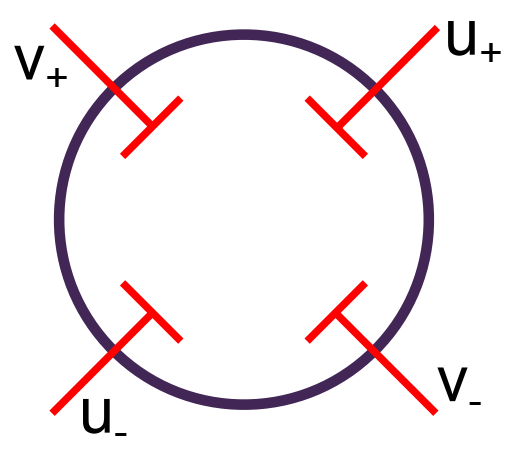
\includegraphics[width=0.5\textwidth]{./setup/fig/bpm.png}
	\caption{The BPM uses four sensing wires to determine the beam position. Since the wires do not actually touch the beam, this measurement can be done during data taking \cite{harp_schem}.}
	\label{fig:bpm}
\end{center}
\end{figure}

The BPM electronics have a phase lag between the BPM measurement and the actual beam position. This means that the BPMs cannot provide position information on an event-by-event basis. However, they do provide a measure of the average position of the beam with a record of beam spread. This information is a critical component to calibrating the raster to provide accurate event-by-event position information.

\subsubsection{Beam Position Monitor Calibration}

Using the BPMs alone provides only a reference position. The BPMs must be calibrated using a harp in order to measure the absolute beam position. This is done by a ``bullseye scan'', shown in Figure \ref{fig:bullseye}. This is accomplished by moving the beam to five positions corresponding to the corners of a square and the center of the square. The harp will give an absolute position measurement of the beam at these positions. The BPMs are also used to measure the beam position as well. The calibration is done by determining the transformation coefficients that will convert the BPM signals to the positions returned by the harps.

\begin{figure}
\begin{center}
	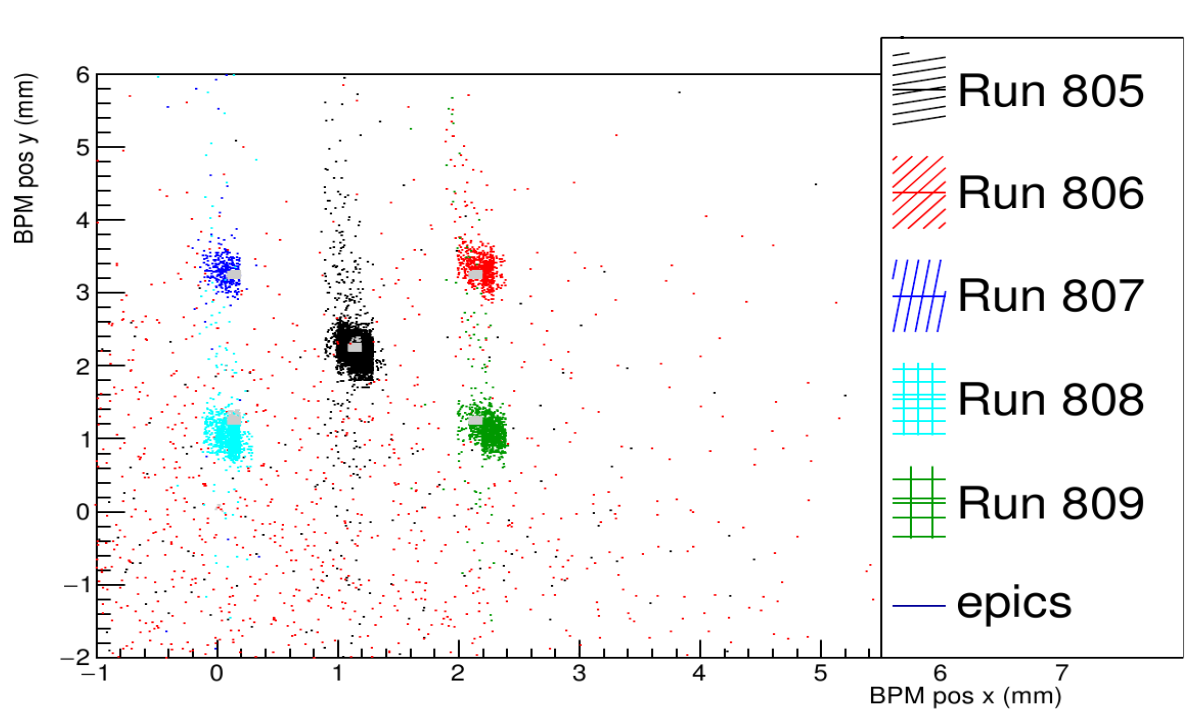
\includegraphics[width=0.7\textwidth]{./setup/fig/bullseye_scan.png}
	\caption{A bullseye scan maps five positions of the beam with the harp, shown as runs 805-809. The BPM calibration is then adjusted to make the reconstructed beam position, shown as gray blocks, match the harp data.}
	\label{fig:bullseye}
\end{center}
\end{figure}